\documentclass[a4paper]{article}

\usepackage[utf8]{inputenc}
\usepackage[portuguese]{babel}
\usepackage{graphicx}
\usepackage[hidelinks]{hyperref}
\usepackage{algorithm}
\usepackage{algpseudocode}
\usepackage{listings}
\usepackage{xcolor}
\usepackage[framemethod=TikZ]{mdframed}
\usepackage{lipsum}

\definecolor{listinggray}{gray}{0.9}
\definecolor{lbcolor}{rgb}{0.9,0.9,0.9}
\lstset{
backgroundcolor=\color{lbcolor},
    tabsize=4,    
%   rulecolor=,
    language=[GNU]C++,
        basicstyle=\scriptsize,
        upquote=true,
        aboveskip={1.5\baselineskip},
        columns=fixed,
        showstringspaces=false,
        extendedchars=false,
        breaklines=true,
        prebreak = \raisebox{0ex}[0ex][0ex]{\ensuremath{\hookleftarrow}},
        frame=single,
        numbers=left,
        showtabs=false,
        showspaces=false,
        showstringspaces=false,
        identifierstyle=\ttfamily,
        keywordstyle=\color[rgb]{0,0,1},
        commentstyle=\color[rgb]{0.026,0.112,0.095},
        stringstyle=\color[rgb]{0.627,0.126,0.941},
        numberstyle=\color[rgb]{0.205, 0.142, 0.73},
%        \lstdefinestyle{C++}{language=C++,style=numbers}’.
}
\lstset{
    backgroundcolor=\color{lbcolor},
    tabsize=4,
  language=C++,
  captionpos=b,
  tabsize=3,
  frame=lines,
  numbers=left,
  numberstyle=\tiny,
  numbersep=5pt,
  breaklines=true,
  showstringspaces=false,
  basicstyle=\footnotesize,
  identifierstyle=\color{magenta},
  keywordstyle=\color[rgb]{0,0,1},
  commentstyle=\color{Darkgreen},
  stringstyle=\color{red}
  }

\mdfdefinestyle{MyFrame}{%
    linecolor=black,
    outerlinewidth=2pt,
    roundcorner=20pt,
    innertopmargin=\baselineskip,
    innerbottommargin=\baselineskip,
    innerrightmargin=20pt,
    innerleftmargin=20pt,
    backgroundcolor=gray!50!white}

\algdef{SE}[DOWHILE]{Do}{doWhile}{\algorithmicdo}[1]{\algorithmicwhile\ #1}%

\graphicspath{ {figures/} }

\bibliography{references}

\begin{titlepage}

\begin{center}

\title {


\includegraphics[scale=0.5]{feup-logo.png}\linebreak\linebreak\linebreak

\Huge\textbf{Paralelização do Algoritmo \textit{The Sieve of Eratosthenes}}\linebreak

\Large\textbf{Relatório}\linebreak

\Large{4º ano do Mestrado Integrado em Engenharia Informática e Computação}\linebreak\linebreak

\Large\textbf{Computação Paralela}\linebreak
}

\large\author{

\textbf{Elementos do grupo:}\\
Henrique Manuel Martins Ferrolho - \href{https://sigarra.up.pt/feup/pt/fest_geral.cursos_list?pv_num_unico=201202772}{201202772} - \href{mailto:ei12079@fe.up.pt}{ei12079@fe.up.pt}\\
João Filipe Figueiredo Pereira - \href{https://sigarra.up.pt/feup/pt/fest_geral.cursos_list?pv_num_unico=201104203}{201104203} - \href{mailto:ei12023@fe.up.pt}{ei12079@fe.up.pt}\\
Leonel Jorge Nogueira Peixoto - \href{https://sigarra.up.pt/feup/pt/fest_geral.cursos_list?pv_num_unico=201204919}{201204919} - \href{mailto:ei12178@fe.up.pt}{ei12079@fe.up.pt}\linebreak\linebreak
}

\Large{Faculdade de Engenharia da Universidade do Porto \\ Rua Roberto Frias, s\/n, 4200-465 Porto, Portugal}\linebreak\linebreak\linebreak

25 de Maio de 2016

\end{center}

\end{titlepage}

\begin{document}

\section{Introdução}

No âmbito da Unidade Curricular de Computação Paralela, foi proposto um estudo da paralelização do algoritmo \textit{The Sieve of Eratosthenes} através do uso de APIs como OpenMP para memória partilhada, e de bibliotecas como OpenMPI para memória distribuída.\\
Neste relatório é descrito o algoritmo proposto, e são discutidas algumas abordagens do mesmo utilizando paralelismo. São ainda apresentadas experiências do desempenho do algoritmo, bem como as suas avaliações e conclusões segundo algumas métricas.

\section{Descrição do Problema}

\textit{The Sieve of Eratosthenes} é um algoritmo simples para encontrar todos os números primos num intervalo [2, $n$] : $n \in \mathbb{N} \setminus \{1\}$. Um número é considerado primo se e só se for divisível por ele próprio e por 1.\\
O objetivo principal deste problema será paralelizar o algoritmo de modo a obter melhor \textit{performance} e escalabilidade para intervalos de grandeza elevada.
 
\section{Algoritmo \textit{The Sieve of Eratosthenes}}

O algoritmo \textit{The Sieve of Eratosthenes} atua sobre uma lista de $n$ números inteiros e consiste em marcar todos os múltiplos dos números primos inferiores ou iguais a $\sqrt{n}$. Os números que não se encontram marcados representam o conjunto de números primos encontrados nesse intervalo.

\begin{figure}[h]
    \centering
    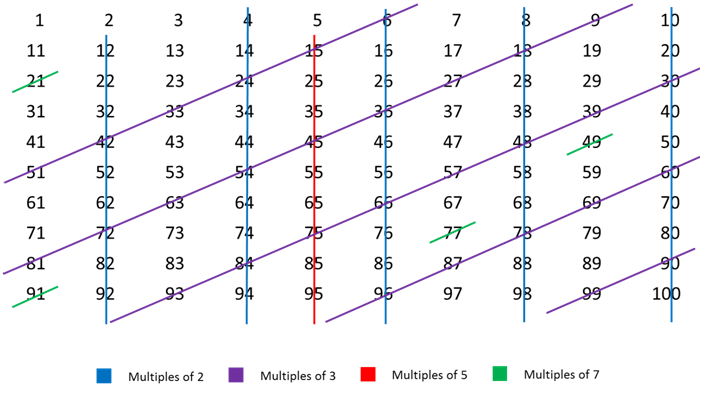
\includegraphics[width=0.75\textwidth]{sieve_example.png}
    \caption{Exemplo do \textit{The Sieve of Eratosthenes.}}
    \label{fig:Sieve}
\end{figure}

As suas complexidades temporal e espacial são $\mathcal{O}(n\ log\ log\ n)$ e $\mathcal{O}(n)$, respetivamente. O pseudo-código é apresentado no \textbf{Algorithm \ref{alg:TheSieveOfEratosthenes}}:

\pagebreak

\begin{algorithm}
\caption{\textit{The Sieve of Eratosthenes}}
\label{alg:TheSieveOfEratosthenes}
\begin{algorithmic}[1]
\State\textbf{input} an integer n $>$ 1
\State\textbf{let} A be an \textbf{array of boolean values}, indexed by \textbf{integers} 2 to n, initially \textbf{all set to true}\linebreak
\For{$i$ = 2, not exceeding $\sqrt{n}$}
\For{$j$ = $i^2$, $i^2+i$, $i^2+2i$, $i^2+3i$, ..., not exceeding $n$}
\State A[$j$] = \textbf{false}
\EndFor
\Do
\State $i$ = $i$ + 1
\doWhile{A[$i$] is \textbf{false and} $i^2 < n$}
\EndFor
\end{algorithmic}
\end{algorithm}
 
\section{Implementação do Algoritmo}
 
Como foi dito na \textbf{Introdução}, foram desenvolvidas algumas implementações do algoritmo para o estudo da \textit{performance} e escalabilidade neste problema: uma versão de memória partilhada, com a \textit{API} \textbf{OpenMP}; e outra versão de memória distribuída, com a bilbioteca \textbf{OpenMPI}. Foi utilizada a linguagem de programação \textbf{C\texttt{++}} para o desenvolvimento de todas as versões.
 
\subsection{Algoritmo Sequencial}
 
Para a versão \textbf{sequencial} do algoritmo, apenas foi necessário implementar o seguinte pseudo-código.

\begin{algorithm}
\caption{Versão \textbf{Sequencial}}
\label{alg:SequentialSieve}
\begin{lstlisting}
for (unsigned long p = 2; pow(p, 2) < size;) {
	for (unsigned long i = pow(p, 2); i < size; i += p)
		list[i] = false;

	do {
		p++;
	} while (!list[p] && pow(p, 2) < size);
}
\end{lstlisting}
\end{algorithm}

O código apresentado em \textbf{Algorithm \ref{alg:SequentialSieve}} pode ser encontrado no ficheiro \textbf{\textit{SequentialSieve.cpp}}, que se encontra na pasta \textbf{\textit{src}} do projeto.
 
\subsection{Paralelização do Algoritmo}
 
Uma das soluções para melhorar a \textit{perfomance} do algoritmo é paralelizar o mesmo. O paralelismo pode ser efetuado de duas formas: partilhando a memória pelo número de \textit{threads} disponíveis no processador (\textbf{OpenMP}); ou dividindo a estrutura de dados utilizada por diferentes processadores, o que possibilita, neste caso, que cada processo tenha memória local não partilhada com os restantes (\textbf{OpenMPI}).

Pode ainda utilizar-se um modelo híbrido com partilha e distribuição de memória.

Para ambos os casos, o paralelismo tem de ser aplicado em blocos de código específicos do algoritmo. Paralelizar tudo não é concebível.

\begin{algorithm}
\caption{Bloco a paralelizar}
\label{alg:Block}
\begin{lstlisting}
for (unsigned long i = p * p; i < size; i += p)
			list[i] = false;
\end{lstlisting}
\end{algorithm}

A marcação dos múltiplos do primo $p$ no intervalo [$p^2$, $size$] foi o bloco escolhido - como é mostrado no \textbf{Algorithm \ref{alg:Block}}.

\subsubsection{Paralelismo com Memória Partilhada - OpenMP}

A versão paralela utilizando a API \textbf{OpenMP} baseia-se na partilha de memória de um processo em execução, pelas diferentes \textit{threads}, concorrentemente.

O \textbf{OpenMP} possui diversas formas de paralelizar um processo. Neste caso, a inserção da linha \textit{pragma omp parallel for} é o necessário para as várias \textit{threads} executarem paralelamente o ciclo pretendido, como se pode verificar no excerto de código apresentado no \textbf{Algorithm \ref{alg:OpenMPSieve}}.

\begin{algorithm}
\caption{Modelo Paralelo com \textbf{OpenMP}}
\label{alg:OpenMPSieve}
\begin{lstlisting}
omp_set_num_threads(threads); // Aplicar o numero de threads especificado

for (unsigned long p = 2; p * p < size;) {

	#pragma omp parallel for // Bloco a paralelizar
	for (unsigned long long i = p * p; i < size; i += p)
		list[i] = false;
	
	do {
		p++;
	} while (!list[p] && p * p < size);
}
\end{lstlisting}
\end{algorithm}

\subsubsection{Versão Paralelizada com Memória Distribuída - OpenMPI}

A versão paralela utilizando a biblioteca \textbf{OpenMPI} baseia-se na distribuição de memória por diferentes processos. Este método é aplicado ao nível da estrutura de dados que é usada no algoritmo: a lista contendo todos os números de [2, $n$] é dividida pelo número de processos a executar. Cada processo terá memória local não partilhada para o seu bloco, e efetuará a marcação dos múltiplos dos números primos no mesmo. O número primo de cada ciclo é dado pelo processo \textit{root} (rank = 0) e é partilhado, através de \textit{broadcast}, aos processos restantes para que estes calculem os seus múltiplos. Após cada ciclo de cálculo, o processo \textit{root} descobre o próximo primo a analisar e volta a partilhá-lo.\\

Para o cálculo do intervalo em cada bloco (\textbf{BLOCK\_SIZE}), e dos seus valores mínimo (\textbf{BLOCK\_LOW}) e máximo (\textbf{BLOCK\_HIGH}), foram definidas \textit{macros} que recebem como parâmetros: o índice do processo, o número de elementos da lista (à exceção do número 1), e o número de processos que irão executar o algoritmo.

\begin{algorithm}
\caption{\textit{Macros} para definir os valores de cada bloco (processo)}
\label{alg:Macros}
\begin{lstlisting}
#define BLOCK_LOW(i, n, p) ((i) * (n) / (p))
#define BLOCK_HIGH(i, n, p) (BLOCK_LOW((i) + 1, n, p) - 1)
#define BLOCK_SIZE(i, n, p) (BLOCK_LOW((i) + 1, n, p) - BLOCK_LOW(i, n, p))
\end{lstlisting}
\end{algorithm}

Nesta versão, é necessário calcular um \textit{start value} para cada bloco no início de cada ciclo. Este valor terá obrigatoriamente de ser múltiplo do primo atual.

\begin{algorithm}
\caption{Modelo Paralelo com \textbf{Open MPI}}
\label{alg:OpenMPISieve}
\begin{lstlisting}
for (unsigned long p = 2; p * p <= n;) {
	// calcular o valor de inicio do bloco para cada processo
	if (p * p < lowValue) {
		lowValue % p == 0 ?
				startBlockValue = lowValue :
				startBlockValue = lowValue + (p - (lowValue % p));
	} else {
		startBlockValue = p * p;
	}

	// marcar os multiplos de cada primo
	for (unsigned long i = startBlockValue; i <= highValue; i += p)
		list[i - lowValue] = false;

	// obter o proximo primo e fazer broadcast para os outros processos
	if (rank == 0) {
		do {
			p++;
		} while (!list[p - lowValue] && p * p < highValue);
	}

	MPI_Bcast(&p, 1, MPI_LONG, 0, MPI_COMM_WORLD);
}
\end{lstlisting}
\end{algorithm}

Como se pode verificar no \textbf{Algorithm \ref{alg:OpenMPISieve}}, se o valor mínimo do bloco for múltiplo do primo atual, então esse valor será o \textit{start value}; caso contrário, é necessário achar o múltiplo mais próximo e atribuí-lo ao valor inicial.

\subsubsection{Versão Paralelizada Híbrida}

A versão de paralelismo híbrida resulta da junção das implementações do \textbf{Algorithm \ref{alg:OpenMPSieve}} (OpenMP) com o \textbf{Algorithm \ref{alg:OpenMPISieve}} (OpenMPI).

A única adição feita neste modelo foi o \textit{pragma omp parallel for} que, assim como no modelo paralelo com \textbf{OpenMP}, servirá para as várias \textit{threads} executarem paralelamente o ciclo pretendido nos diferentes processos.

\begin{algorithm}
\caption{Modelo Híbrido com \textbf{OpenMPI} e \textbf{OpenMP} - Adição de \textit{pragma}}
\label{alg:OpenMPIOpenMPSieve}
\begin{lstlisting}
    omp_set_num_threads(threads); // Alocar numero de threads pretendidas
    
    ...

    #pragma omp parallel for // ciclo a paralelizar
	for (unsigned long i = startBlockValue; i <= highValue; i += p)
		list[i - lowValue] = false;
\end{lstlisting}
\end{algorithm}

\section{Experiências e Análise dos Resultados}
 
\subsection{Descrição das Experiências}

Nesta secção são apresentados os resultados obtidos para as diversas experiências realizadas com as diferentes versões do algoritmo.\\

Para as experiências utilizaram-se intervalos de grande escala, nomeadamente, potências de 2 com expoente a variar de 25 a 32: $2^i$, $i \in [25, 32]$. Nos modelos paralelos foram adicionados outros fatores como: o número de processos a utilizar, no caso de modelo de memória distribuída (\textbf{OpenMPI}); o número de \textit{threads}, no caso de modelo de memória partilhada (\textbf{OpenMP}); ambos os anteriores, como no caso do modelo híbrido.\\

Cada experiência foi realizada em quatro computadores, variando o número de processos disponíveis em cada computador a partir do ficheiro \textit{hostfile}.\\

\begin{mdframed}[style=MyFrame]
\begin{center}
\caption{Exemplo do ficheiro \textit{hosfile}\\}
192.168.32.151 cpu=1 || 2 || 4 || 8\\
192.168.32.152 cpu=1 || 2 || 4 || 8\\
192.168.32.153 cpu=1 || 2 || 4 || 8\\
192.168.32.150 cpu=1 || 2 || 4 || 8\\
\end{center}
\end{mdframed}

Os processos permitidos nos computadores variaram entre 1, 2, 4, e 8 processos, permitindo um número total de processos quatro vezes superior aos permitidos (\textbf{Equação \ref{eq:1}}), e o número de \textit{threads} entre 1 e 8, inclusive.
\begin{equation}
\label{eq:1}
Nº Total Processos = 4 Computadores * Nº Processos Permitidos
\end{equation}

As características dos computadores utilizados nas experiências são as seguintes:
\begin{enumerate}
\item \textbf{Modelo Processador:} Intel(R) Core™ i7-4790 CPU @ 3.60GHz
\item \textbf{Nº de Processadores:} 8
\item \textbf{\textit{Cache}}:
\begin{enumerate}
\item 4 \textit{caches} de dados L1 de 32KB
\item 4 \textit{caches} de dados/instruções L2 de 256KB
\item 1 \textit{cache} de dados/intruções L3 de 8MB
\end{enumerate}
\item \textbf{Memória RAM total:} 16342672 KB
\end{enumerate}  


\subsection{Metodologia de Avaliação}

Além das variáveis referidas na secção anterior, foi ainda medido o tempo de execução de cada experiência. O tempo de execução é usado para o cálculo das métricas de \textit{performance} e escalabilidade.\\

As \textbf{métricas de \textit{performance}} utilizadas são: o \textbf{\textit{speedup}} em função da dimensão de dados ($n$), o número de instruções por segundo (\textbf{\textit{OP/s}}), e a \textbf{eficiência} em função do número de processadores utilizados.\\

O \textbf{\textit{speedup}} é calculado em função do tempo de execução obtido na versão sequencial, como é apresentado na \textbf{Equação \ref{eq:2}}. $T_{paralelo}$ representa os tempos obtidos em qualquer das versões paralelas.

\begin{equation}
\label{eq:2}
    Speedup = \frac{T_{sequancial}}{T_{paralelo}}
\end{equation}
\\

O número de instruções por segundo, \textbf{\textit{OP/s}}, é obtido através da complexidade temporal do algoritmo, como é possível observar na \textbf{Equação \ref{eq:3}}. $T_i$ corresponde ao tempo de execução obtido em cada experiência.

\begin{equation}
\label{eq:3}
    OP/s(i) = \frac{n\ log\ log\ n}{T_i}
\end{equation}
\\

A \textbf{eficiência} é o rácio de utilização dos processadores na execução do programa em paralelo - \textbf{Equação \ref{eq:4}}. $P$ representa o número de processadores utilizados.

\begin{equation}
\label{eq:4}
    E = \frac{Speedup}{P}
\end{equation}
\\

Esta métrica servirá para concluir a escalabilidade das diferentes versões do algoritmo, sendo que um modelo é escalável se $E \in [0, 1]$ com $P$ e $n$ a aumentarem.


\pagebreak


\subsection{Análise dos Resultados}
 
\subsubsection{Versão Sequencial}

Os resultados obtidos para a versão sequencial do algoritmo são apresentados na coluna \textbf{Seq.} da \textbf{Tabela \ref{tab:1}}.

Pode concluir-se que o tempo decorrido aumenta em função do intervalo dado. Note-se ainda que esse aumento é próximo do factor 2 (um dado tempo decorrido é, aproximadamente, o dobro do tempo decorrido anterior), que corresponde também ao aumento da dimensão do intervalo de primos a serem gerados.

\begin{table}[h]
\centering
\begin{tabular}{||c|c|c|c|c|c||}
\hline
\multirow{Expoente} & \multirow{Seq.} & \multicolumn{4}{c||}{Paralelo - Memória Partilhada} \\ \cline{3-6} 
                   &                       & 2           & 4           & 6          & 8          \\ \hline
25                 & 0.292                 & 0.219       & 0.173       & 0.207      & 0.373      \\ \hline
26                 & 0.508                 & 0.436       & 0.401       & 0.434      & 0.440      \\ \hline
27                 & 1.107                 & 0.945       & 0.873       & 0.910      & 0.999      \\ \hline
28                 & 2.320                 & 1.891       & 1.855       & 1.915      & 2.024      \\ \hline
29                 & 4.881                 & 3.956       & 4.196       & 4.007      & 4.082      \\ \hline
30                 & 10.162                & 8.156       & 8.069       & 8.325      & 8.442      \\ \hline
31                 & 21.160                & 16.980      & 16.932      & 17.101     & 17.306     \\ \hline
32                 & 43.412                & 35.099      & 34.872      & 35.583     & 35.769     \\ \hline
\end{tabular}
\caption{Tempos de execução (segundos) da versão sequencial e da versão paralela com memória partilhada.}
\label{tab:1}
\end{table}

No que diz respeito à \textit{performance} desta versão, podemos verificar um decréscimo no número de operações por segundo - \textbf{Figura \ref{fig:sequentialPerformance}}. Esse decréscimo deve-se a uma gestão de memória mais intensiva, consequente do aumento exponencial do tamanho da lista de primos a processar. 

\begin{figure}[h]
    \begin{center}
    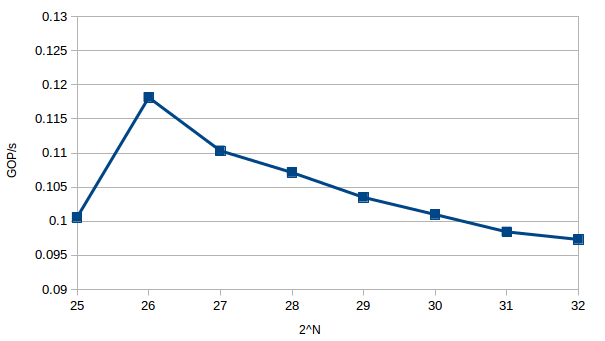
\includegraphics[width=0.9\textwidth]{sequentialPerformance.png}
    \caption{Performance da versão \textit{sequencial} do algoritmo.}
    \label{fig:sequentialPerformance}
    \end{center}
\end{figure}
\pagebreak

\subsubsection{Versão de Memória Partilhada - OpenMP}

Os resultados obtidos para o modelo de memória partilhada são apresentados na \textbf{Tabela \ref{tab:1}}, juntamente com os resultados da versão sequencial. Os valores apresentados dizem respeito a um número par de \textit{threads}.\\
A experiência que originou melhores resultados foi a que usou quatro \textit{threads}. Verificou-se ainda que um número de \textit{threads} superior ao número de \textit{cores} físicos não melhorou os resultados.\\

\begin{figure}[h]
    \centering
    \hspace*{-0.7in}
    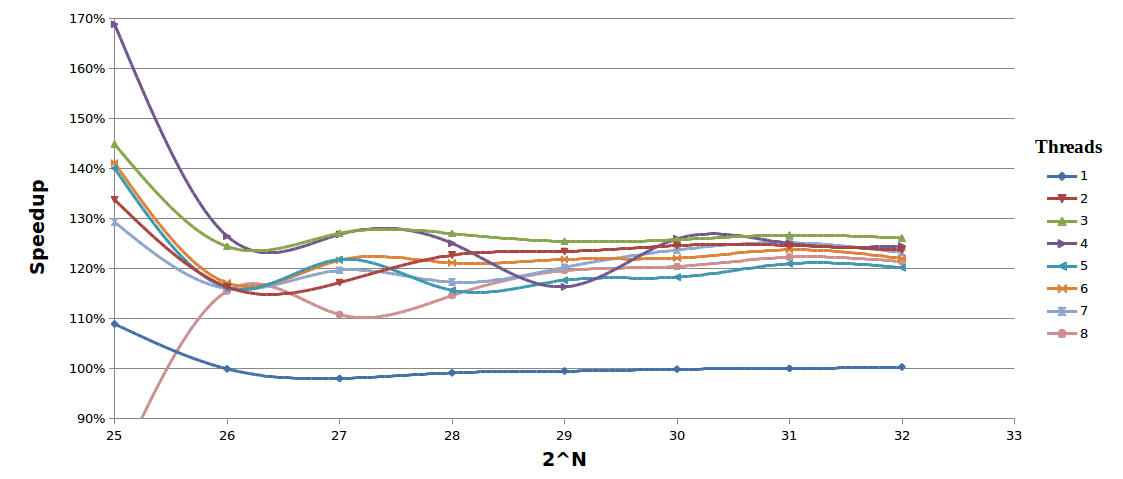
\includegraphics[width=1.3\textwidth]{openMPSpeedup.png}
    \caption{\textit{Speedup} da versão paralela com memória partilhada em relação à versão sequencial do algoritmo.}}
    \label{fig:speedupOpenMP}
\end{figure}

Com base na \textbf{Figura 3}, conclui-se que o \textit{speedup} calculado, em comparação com a versão sequencial, apresenta melhores resultados com o uso de 4 \textit{threads} (tal como nos tempos de execução).

Novamente, o uso de um número de \textit{threads} superior a 4 piora os tempos de execução. Para esses tempos de execução, o \textit{speedup} calculado até chega a ser pior que o uso de 2 \textit{threads}.

Note-se ainda que, quando o número de threads utilizadas é superior a 1, o \textit{speedup} tende para um valor entre [120\%, 130\%].

\subsubsection{Modelo de Memória Distribuída}

Os resultados para o modelo paralelo de memória distribuída foram obtidos a partir de 4 experiências: 1 processo em cada computador (4 no total), 2 processos em cada computador (8 no total), 4 processos em cada computador (16 no total) e 8 processos em cada computador (32 no total).

Os \textit{speedups} calculados são apresentados na \textbf{Figura 4}.

\pagebreak

\begin{figure}[h]
    \centering
    \hspace*{-0.8in}
    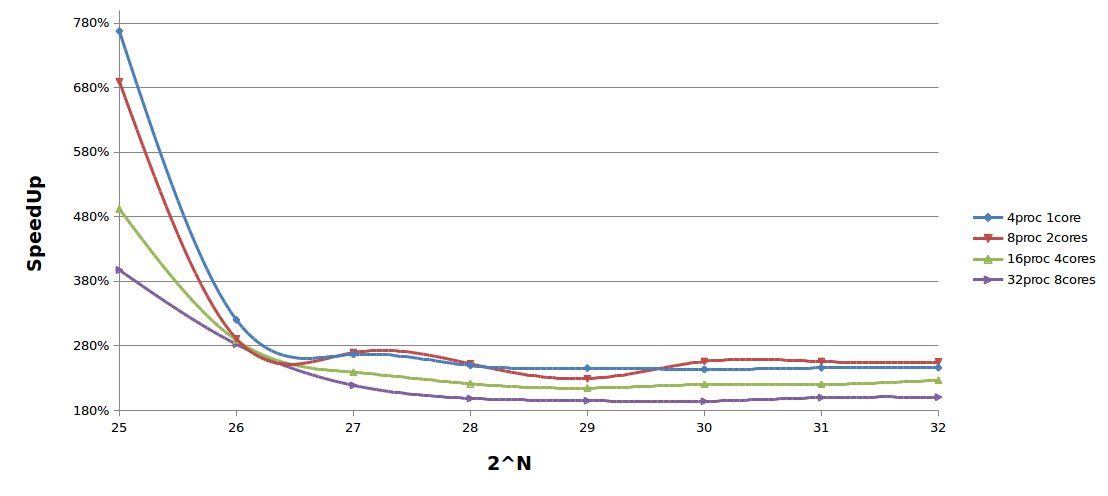
\includegraphics[width=1.3\textwidth]{openMPISpeedup.png}
    \caption{\textit{Speedup} da versão paralela com memória distribuída em relação à versão sequencial do algoritmo}}
    \label{fig:MPI}
\end{figure}

Analisando os valores do \textit{speedup} obtidos, é possível verificar que a paralelização do processo de cálculo com o modelo de memória distribuída apresenta valores bastante mais elevados do que aqueles obtidos com o modelo de memória partilhada. De facto, na \textbf{Figura 3}, em média, o \textit{speedup} para a versão de memória partilhada é de 125\%, enquanto que, para a versão de memória distribuída, é de 240\% (apesar de se verificar um maior \textit{speedup} para \textit{n} = 25).

Conclui-se ainda que o aumento do número de processos não leva ao aumento do \textit{speedup}. Os valores ótimos foram obtidos com 2 processos em cada computador, levando a um total de 8 processos sobre os 32 disponíveis.

\begin{table}[h]
\centering
\begin{tabular}{|l|l|l|l|l|l|l|l|}
\hline
\multicolumn{8}{|c|}{\textbf{GOP/s (2 processos em cada computador)}}                                                                                                                                                                                     \\ \hline
\textbf{N}  & \multicolumn{1}{c|}{\textbf{2}} & \multicolumn{1}{c|}{\textbf{3}} & \multicolumn{1}{c|}{\textbf{4}} & \multicolumn{1}{c|}{\textbf{5}} & \multicolumn{1}{c|}{\textbf{6}} & \multicolumn{1}{c|}{\textbf{7}} & \multicolumn{1}{c|}{\textbf{8}} \\ \hline
\textbf{25} & 0.145                           & 0.235                           & 0.232                           & 0.429                           & 0.205                           & 0.499                           & 0.694                           \\ \hline
\textbf{26} & 0.130                           & 0.179                           & 0.197                           & 0.249                           & 0.292                           & 0.353                           & 0.344                           \\ \hline
\textbf{27} & 0.121                           & 0.161                           & 0.176                           & 0.219                           & 0.241                           & 0.280                           & 0.297                           \\ \hline
\textbf{28} & 0.116                           & 0.130                           & 0.168                           & 0.183                           & 0.225                           & 0.256                           & 0.270                           \\ \hline
\textbf{29} & 0.113                           & 0.147                           & 0.163                           & 0.196                           & 0.214                           & 0.243                           & 0.237                           \\ \hline
\textbf{30} & \multicolumn{1}{c|}{0.111}      & \multicolumn{1}{c|}{0.146}      & \multicolumn{1}{c|}{0.160}      & \multicolumn{1}{c|}{0.170}      & \multicolumn{1}{c|}{0.175}      & \multicolumn{1}{c|}{0.190}      & \multicolumn{1}{c|}{0.258}      \\ \hline
\textbf{31} & 0.109                           & 0.143                           & 0.157                           & 0.189                           & 0.184                           & 0.232                           & 0.252                           \\ \hline
\textbf{32} & 0.106                           & 0.142                           & 0.155                           & 0.187                           & 0.190                           & 0.222                           & 0.248                           \\ \hline
\end{tabular}
\caption{GOP/s para o modelo de memória distribuída.}
\label{tab:2}
\end{table}

Com base na \textbf{Tabela \ref{tab:2}}, podemos observar um grande aumento no número de operações por segundo relativamente à versão sequencial. Esse aumento é um dos fatores para a melhoria dos tempos de execução.\\

Relativamente à \textbf{eficiência} desta versão pode-se verificar que os valores se encontram todos no intervalo $[0, 1]$ (à exceção de $2^{25}$ para um processo em cada computador).\\

Com esta análise, podemos concluir que esta versão é \textbf{escalável} para problemas de maiores dimensões.\\

\begin{table}[h]
\centering
\begin{tabular}{|c|l|l|l|l|l|}
\hline
\multicolumn{6}{|c|}{\textbf{Eficiência no modelo de memória distribuída}} \\ \hline
\multicolumn{6}{|c|}{\textbf{P}}                                 \\ \hline
\multirow{\textbf{N}} &    & 4     & 8     & 16    & 32    \\ \cline{2-6} 
                              & 25   & 1.325   & 0.595   & 0.212  & 0.086  \\ \cline{2-6} 
                              & 26   & 0.644   & 0.292   & 0.145  & 0.071  \\ \cline{2-6} 
                              & 27   & 0.525   & 0.265   & 0.118  & 0.054  \\ \cline{2-6} 
                              & 28   & 0.491   & 0.248   & 0.109  & 0.049  \\ \cline{2-6} 
                              & 29   & 0.490   & 0.228   & 0.107  & 0.049  \\ \cline{2-6} 
                              & 30   & 0.484   & 0.254   & 0.109  & 0.048  \\ \cline{2-6} 
                              & 31   & 0.485   & 0.252   & 0.109  & 0.049  \\ \cline{2-6} 
                              & 32   & 0.488   & 0.253   & 0.112  & 0.050  \\ \hline
\end{tabular}
\caption{Eficiência obtida para o modelo de memória distribuída.}
\label{tab:3}
\end{table}


\subsubsection{Modelo híbrido}

Os resultados deste modelo foram obtidos a partir de vários testes, em que se fez variar o número de processos e \textit{threads} em cada computador. É possível visualizar os \textit{speedups} na \textbf{Figura \ref{fig:MPI&OMP}}.

\begin{figure}[h]
    \centering
    \hspace*{-0.8in}
    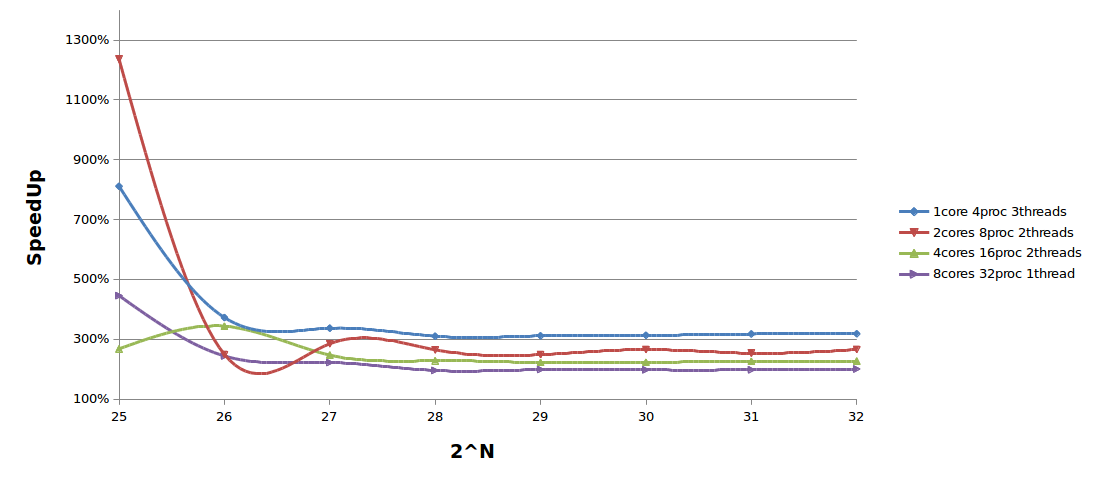
\includegraphics[width=1.3\textwidth]{openMPIOMPSpeedup.png}
    \caption{\textit{Speedup} da versão híbrida com memória distribuída e memória partilhada em relação à versão sequencial do algoritmo.}
    \label{fig:MPI&OMP}
\end{figure}

\pagebreak

Conjugando os modelos de memória partilhada e memória distribuída, obtiveram-se valores de \textit{speedup} relativamente superiores aos do modelo de memória partilhada (300\% vs 240\% em média).

Tal como no modelo de memória partilhada, o aumento do número de processos e \textit{threads} não leva ao aumento do \textit{speedup}, pois neste modelo, os valores ótimos foram obtidos com 1 processo de 3 \textit{threads} em cada computador - totalizando 12 \textit{threads} sobre os 32 disponíveis.

\begin{table}[h]
\centering
\begin{tabular}{|c|l|l|l|l|l|}
\hline
\multicolumn{6}{|c|}{\textbf{Eficiência no modelo de híbrido}}   \\ \hline
\multicolumn{6}{|c|}{\textbf{P}}                                 \\ \hline
\multirow{\textbf{N}} &    & 4     & 8     & 16    & 32    \\ \cline{2-6} 
                            & 25 & 2.028 & 1.545 & 0.168 & 0.139 \\ \cline{2-6} 
                            & 26 & 0.931 & 0.312 & 0.215 & 0.076 \\ \cline{2-6} 
                            & 27 & 0.842 & 0.356 & 0.154 & 0.069 \\ \cline{2-6} 
                            & 28 & 0.775 & 0.331 & 0.143 & 0.061 \\ \cline{2-6} 
                            & 29 & 0.779 & 0.311 & 0.139 & 0.062 \\ \cline{2-6} 
                            & 30 & 0.783 & 0.332 & 0.139 & 0.062 \\ \cline{2-6} 
                            & 31 & 0.794 & 0.317 & 0.141 & 0.062 \\ \cline{2-6} 
                            & 32 & 0.796 & 0.333 & 0.142 & 0.063 \\ \hline
\end{tabular}
\caption{Eficiência obtida para o modelo híbrido.}
\label{tab:4}
\end{table}

Assim como no modelo de memória distribuída, a análise da eficiência através da \textbf{Tabela \ref{tab:4}} permite-nos concluir que esta versão é \textbf{escalável} a problemas maiores, uma vez que os valores apresentados estão, maioritariamente, entre o intervalo $[0, 1]$.

\section{Conclusões}

Com este trabalho foi possível conhecer e aplicar conhecimentos sobre a \textit{API} de paralelização \textit{OpenMP} e a biblioteca \textit{OpenMPI}.

Foram implementados três modelos diferentes de forma a paralelizar a geração de números primos pelo algoritmo \textit{The Sieve of Eratosthenes}.

Após a análise de cada modelo, é possível concluir que o uso de memória distribuída por vários computadores é mais vantajosa que o uso de memória partilhada num único computador. Para além de ser mais vantajosa, é também mais económica, pois a criação de \textit{clusters} a partir de computadores comuns pode revelar-se menos dispendiosa do que a aquisição de um único computador de processamento de alta performance com muitos \textit{cores}.

Finalmente, conclui-se também que a combinação dos modelos de memória partilhada e distribuída apresenta ainda mais vantagens do que o uso de um desses modelos isolado.

%%\printbibliography

\end{document}